
\documentclass[oneside,12pt,numbers,spanish]{ezthesis}
%% # Opciones disponibles para el documento #
%%
%% Las opciones con un (*) son las opciones predeterminadas.
%%
%% Modo de compilar:
%%   draft            - borrador con marcas de fecha y sin im'agenes
%%   draftmarks       - borrador con marcas de fecha y con im'agenes
%%   final (*)        - version final de la tesis
%%
%% Tama'no de papel:
%%   letterpaper (*)  - tama'no carta (Am'erica)
 %%   a4paper          - tama'no A4    (Europa)
%%
%% Formato de impresi'on:
%%   oneside          - hojas impresas por un solo lado
%%   twoside (*)      - hijas impresas por ambos lados
%%
%% Tama'no de letra:
%%   10pt, 11pt, o 12pt (*)
%%
%% Espaciado entre renglones:
%%   singlespace      - espacio sencillo
%%   onehalfspace (*) - espacio de 1.5
%%   doublespace      - a doble espacio
%%
%% Formato de las referencias bibliogr'aficas:
%%   numbers          - numeradas, p.e. [1]
%%   authoryear (*)   - por autor y a'no, p.e. (Newton, 1997)
%%
%% Opciones adicionales:
%%   spanish         - tesis escrita en espa'nol
%%
%% Desactivar opciones especiales:
%%   nobibtoc   - no incluir la bibiolgraf'ia en el 'Indice general
%%   nofancyhdr - no incluir "fancyhdr" para producir los encabezados
%%   nocolors   - no incluir "xcolor" para producir ligas con colores
%%   nographicx - no incluir "graphicx" para insertar gr'aficos
%%   nonatbib   - no incluir "natbib" para administrar la bibliograf'ia

%% Paquetes adicionales requeridos se pueden agregar tambi'en aqu'i.
%% Por ejemplo:
\usepackage[spanish]{babel}
\usepackage{cite}
\usepackage{natbib} 
\usepackage{subfig}
\usepackage[utf8x]{inputenc}
\usepackage{multicol}
\usepackage{multirow, array}
\usepackage{graphicx} 
\usepackage{float}  
\usepackage{amsmath}
\usepackage{amssymb}
\usepackage{pgfgantt }



%% # Datos del documento #
%%\documentclass[12pt]{•}%% Nota que los acentos se deben escribir: \'a, \'e, \'i, etc.
%% La letra n con tilde es: \~n.

\author{Ghabriel Villarreal}
\title{Paquete en lenguaje R, para la simulacion del modelo MOMOS}
\supervisor{Rossana Timaure}
\institution{Universidad Nacional Experimental del T\'achira}
\faculty{Vicerectorado Acad\'emico}
\department{Departamento de Ingenier\'ia en Inform\'atica}

%% # M'argenes del documento #
%% 
%% Quitar el comentario en la siguiente linea para austar los m'argenes del
%% documento. Leer la documentaci'on de "geometry" para m'as informaci'on.

\geometry{left=2cm,right=2cm,top=3cm,bottom=3cm}

%% El siguiente comando agrega ligas activas en el documento para las
%% referencias cruzadas y citas bibliogr'aficas. Tiene que ser *la 'ultima*
%% instrucci'on antes de \begin{document}.
\hyperlinking
\begin{document}

%% En esta secci'on se describe la estructura del documento de la tesis.
%% Consulta los reglamentos de tu universidad para determinar el orden
%% y la cantidad de secciones que debes de incluir.

%% # Portada de la tesis #
%% Mirar el archivo "titlepage.tex" para los detalles.
%% ## Construye tu propia portada ##
%% 
%% Una portada se conforma por una secuencia de "Blocks" que incluyen
%% piezas individuales de informaci'on. Un "Block" puede incluir, por
%% ejemplo, el t'itulo del documento, una im'agen (logotipo de la universidad),
%% el nombre del autor, nombre del supervisor, u cualquier otra pieza de
%% informaci'on.
%%
%% Cada "Block" aparece centrado horizontalmente en la p'agina y,
%% verticalmente, todos los "Blocks" se distruyen de manera uniforme 
%% a lo largo de p'agina.
%%
%% Nota tambi'en que, dentro de un mismo "Block" se pueden cortar
%% lineas usando el comando \\
%%
%% El tama'no del texto dentro de un "Block" se puede modificar usando uno de
%% los comandos:
%%   \small      \LARGE
%%   \large      \huge
%%   \Large      \Huge
%%
%% Y el tipo de letra se puede modificar usando:
%%   \bfseries - negritas
%%   \itshape  - it'alicas
%%   \scshape  - small caps
%%   \slshape  - slanted
%%   \sffamily - sans serif
%%
%% Para producir plantillas generales, la informaci'on que ha sido inclu'ida
%% en el archivo principal "tesis.tex" se puede accesar aqu'i usando:
%%   \insertauthor
%%   \inserttitle
%%   \insertsupervisor
%%   \insertinstitution
%%   \insertdegree
%%   \insertfaculty
%%   \insertdepartment
%%   \insertsubmitdate

\begin{titlepage}
  \TitleBlock{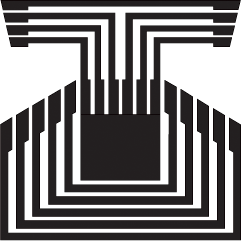
\includegraphics[scale=0.2]{unet.jpg} }  
  \TitleBlock{\small\insertinstitution}
  \TitleBlock[\small\bigskip]{\insertfaculty}
  \TitleBlock[\small\bigskip]{Decanato de Docencia}
  \TitleBlock[\small\bigskip]{\insertdepartment}
  \TitleBlock[\small\bigskip]{Trabajo de aplicaci\'on profesional}
  \TitleBlock[\small\bigskip]{Proyecto especial de grado}
    
 \TitleBlock{\scshape\inserttitle}
 
 \begin{flushright}
  \TitleBlock{ \small Autor:  \insertauthor} 
  \TitleBlock{ \small C.I.:22.676.954 }
  \TitleBlock{ \small ghabriel.villarreal@unet.edu.ve}
  \TitleBlock{\small Tutor(es):  \insertsupervisor}
  \TitleBlock{ \small rttg@unet.edu.ve}
 \end{flushright}
  \TitleBlock{\small San Crist\'obal, Abril de \insertsubmitdate}
  
\end{titlepage}

%% Nota 1:
%% Se puede agregar un escudo o logotipo en un "Block" como:
%%   \TitleBlock{\includegraphics[height=4cm]{escudo_uni}}
%% y teniendo un archivo "escudo_uni.pdf", "escudo_uni.png" o "escudo_uni.jpg"
%% en alg'un lugar donde LaTeX lo pueda encontrar.

%% Nota 2:
%% Normalmente, el espacio entre "Blocks" se extiende de modo que el
%% contenido se reparte uniformemente sobre toda la p'agina. Este
%% comportamiento se puede modificar para mantener fijo, por ejemplo, el
%% espacio entre un par de "Blocks". Escribiendo:
%%   \TitleBlock{Bloque 1}
%%   \TitleBlock[\bigskip]{Bloque2}
%% se deja un espacio "grande" y de tama~no fijo entre el bloque 1 y 2.
%% Adem'as de \bigskip est'an tambi'en \smallskip y \medskip. Si necesitas
%% aun m'as control puedes usar tambi'en, por ejemplo, \vspace*{2cm}.




% \tableofcontents
% \listoffigures
\include{intro}
\chapter{Preliminares}

\section{Planteamiento y formulaci\'on del problema}
La materia orgánica estable del suelo (MOS) se caracteriza por ser el resultado del proceso de descomposición de los residuos de animales y vegetales, los cuales varían en proporción y estado. Estos residuos son sustancias que contribuyen a la fertilidad del suelo, por lo que,  la materia org\'anica del suelo MOS, viene a ser uno de los factores de importancia que determina localidad de un suelo.\\

La descomposición de la materia orgánica es un proceso biológico que ocurre naturalmente, por efecto de diferentes grupos de organismos, entre los cuales destacan los microorganismos del suelo, que permiten transformar los diferentes residuos, en nutrientes básicos y energía. Siendo que una de las funciones MOS es actuar como depósito de carbono, permitiendo que exista en el suelo más del doble del carbono contenido en la atmósfera, por lo que los cambios que experimente está, pueden tener un impacto en el equilibrio global, y por lo tanto un efecto sobre las condiciones climáticas del planeta, al ser considerado el carbono que sale de esta como CO2, el cual es uno de los gases que contribuyen al efecto invernadero del planeta y al cambio climático (IPCC, 2000).\\

En la actualidad, se reporta un incremento en el cambio climático por efecto del impacto antropogénico, el cual se observa en el aumento de la temperatura en diferentes regiones, y como efecto de retroalimentación la temperatura influye sobre el proceso de descomposición y por lo tanto en el almacenamiento de carbono en el suelo y en la vegetación (Andriulo, 2006), todo esto muestra que el suelo es un compartimiento complejo debido a todas las interrelaciones que existen en el mismo.\\

Por lo que la comprensión de los diferentes procesos y transformaciones que ocurren en el suelo, son de gran importancia, sin embargo la cantidad de información que puede ser recolectada, así como la variabilidad en la misma, constituyen un desafío en sí, por lo cual esto conlleva ha utilizar herramientas tecnológicas que permitan el manejo de la información obtenida, es por ello que existe una gran cantidad de modelos que simulan y describen los procesos de la descomposición de la MOS, y los cuales pueden o están siendo acoplados a modelos de pronósticos a nivel global, de igual manera estos modelos están evolucionando, en la búsqueda de una mejor comprensión de los diversos procesos físico, químicos y biológicos [Larionova et al., 2007; Lomander et al., 1998].\\

Existen una gran cantidad de modelos que estudian la MOS, muchos de los cuales están desarrollados sobre plataformas propias, lo cual nos permite el proceso de enseñanza-aprendizaje, así como, de investigación en el desarrollo de mejoras al mismo por otros investigadores, de igual manera existen herramientas donde se han desarrollado de manera práctica modelos, tales como por ejemplo el modelo MOMOS (Materia Organica y MicroOrganismos del Suelo), el cual ha sido calibrado y validado con datos e información de un estudio en un gradiente altitudinal tropical [Pansu et al., 2010, 2014] mostrando buenos resultados en las diferentes evaluaciones, este mismo modelo ha sido evaluado, encontrando una propuesta de evolución del mismos (Valery, 2018). Sin embargo, las investigaciones antes mencionadas, presenta la desventaja de haber sido desarrolladas en un software de simulación privativo llamado Vensim creado por Ventana Systems, Inc. para la construcción de modelos de sistemas dinámicos, limitado a funciones desarrolladas por dicha empresa, lo que no permite ampliar la investigación en otros aspectos de interés sin la necesidad de acudir a otros softwares externos.\\

De igual manera, el grupo de Investigación en Biotecnología Agrícola y Ambiental (GIBAA) de la UNET, ha desarrollado diversos planteamientos de modelos bajo un software libre, por lo que se propone el uso de la herramienta para el análisis estadístico y gráfica llamado R, el cual es un ambiente de programación formado por un conjunto de herramientas muy flexibles que pueden ampliarse fácilmente mediante paquetes, librerías o definiendo nuestras propias funciones. Además, es gratuito y de código abierto. Cualquier usuario puede descargar y crear su código de manera gratuita, sin restricciones de uso, la única regla es que la distribución siempre sea libre (GPL). Gracias a que puede accederse libremente a su código, R no tiene limitadas sus funciones, al contrario de lo que sucede con otras herramientas comerciales. \\

La finalidad de esta investigación consiste en utilizar el modelo MOMOS desarrollado por Valery (2018) en Vensim e implementarlo en R, permitiendo la comparación de los resultados obtenidos en Vensim (Valery, 2018) contra el resultado del paquete a desarrollar. Buscando como meta la versatilidad a los investigadores interesados de poder trabajar sobre un ambiente que puedan manejar y modificar en las diferentes necesidades de trabajo.\\




\section{Objetivos}

\subsection{Objetivo General}
Desarrollar un paquete en el lenguaje R que implemente el modelo MOMOS.


\subsection{Objetivos Espec\'ificos}

\begin{itemize}
\item Estudiar la Estructura del modelo MOMOS.\\
\item Crear las funciones primarias en el lenguaje R para implementar el modelo MOMOS.\\
\item Realizar las pruebas unitarias y funcionales del paquete creado en el lenguaje R.\\
\end{itemize}

\section{Justificaci\'on e Importancia}

En las ciencias agronómicas y áreas afines, en la última década, se han utilizado una serie de herramientas que permiten mejorar los procesos de producción, así como del manejo de los recursos, entre las mismas, se encuentran los modelos dinámicos de simulación los cuales lográn mostrar una representación lo más cercana a la realidad, generando un mejor entendimiento de los procesos en los ecosistemas y agroecosistemas. \\

\section{Alcance y Limitaciones}

El paquete a desarrollar en el lenguaje R permitirá simular el modelo MOMOS, el resultado obtenido se comparará con los obtenidos por Valery (2018) en el programa VENSIM para simular el mismo modelo. \\

\chapter{Fundamentos Te\'oricos}

\section{Antecedentes}

Contreras (2018)  construy\'o: “DimBio, Paquete en lenguaje R para la discrminizaci\'on de modelos de simulaci\'on din\'amicos para procesos biol\'ogicos.”, en este trabajo se expone de forma detallada la realizaci\'on de un paquete en lenguaje R, para la discriminaci\'on de modelos de simulaci\'on din\'amicos para procesos biol\'ogicos, para unificar los estad\'isticos que evaluan el desempeño de los modelos din\'amicos, mediante el c\'alculo para discrimaci\'on de estad\'isticos univariantes y multivariantes utilizados para encontrar un modelo adecuado o que mejor se ajustar\'a al proceso de estudio basado en modelos.\\ 

La investigaci\'on fue de relavancia para este trabajo de grado, ya que en ella crearon un paquete en R, y utilizaron modelos de simulaci\'on din\'amicos.\\

Darghan (2018) realiz\'o: “CGR, Paquete en lenguaje R, para el cálculo de índices fisiológicos de crecimiento y componentes del rendimiento en plantas.” trabajo en el cual se expone el desarrollo del paquete CGR cuyo interés radicó en el cálculo de aquellos índices que dependen de la primera derivada de la forma funcional ajustada al modelo de crecimiento de las plantas, también permite el cálculo de índices instantáneos en cualquier punto de interés por el usuario dentro de la región experimental o dentro del dominio de la función ajustada.\\

La investigaci\'on citada fue tomada como referencia, puesto que realizó cálculos de índices para evaluar el comportamiento de ciertas variables en procesos biol\'ogicos, en este caso, el crecimiento. Lo cual est\'a vinculado al contexto biol\'ogico de los datos que fueron evaluados por el paquete que se desarroll\'o.\\

Ablan (2011) construy\'o: “Una librer\'ia en R para validaci\'on de modelos de simulaci\'on”, en este trabajo se manejaron m\'etodos para la validaci\'on de modelos de simulaci\'on continua para evaluar la calidad del modelo comparando los resultados de series temporales de datos reales con los resultados o salidas obtenidos de una simulaci\'on para el mismo lapso temporal, en el cual se utilizaron los criterios o \'indices de validaci\'on que pueden ser usados para la comparaci\'on de datos y resultados de un modelo, los cuales fueron: el error cuadr\'atico medio, el estad\'isticos de Theil, el error absoluto medio, el \'indice de acuerdo de Willmott, la eficiencia del modelo de Nash Sutcliffe, el coeficiente de correlaci\'on de Pearson, el coeficiente de determinaci\'on, la prueba F, la prueba t pareada, el estad\'istico Hotelling T2, el criterio de informaci\'on de Akaike y la inferencia bayesiana. Con estos criterios o \'indices se cre\'o una librer\'ia del programa estad\'istico R que permiti\'o el uso de estos \'indices para la validaci\'on de modelos de simulaci\'on.\\

La investigaci\'on fue importante en este trabajo de grado, ya que en ella crearon una librer\'ia de R, y utilizaron m\'etodos estad\'isticos para respuesta univariante que son utilizados para la comparaci\'on de datos reales contra datos de modelos de simulaci\'on.\\

\section{Bases Te\'oricas}

\section{Modelos}

En la actualidad el avance de la tecnolog\'ia, permite que para el estudio de sistemas biol\'ogicos,  los modelos de simulaci\'on sean una herramienta que ayuda en el manejo de la informaci\'on, as\'i como la evaluaci\'on y planificaci\'on de manejos y dise\~no de experimentos.\\

Existe una gran cantidad de modelos biol\'ogicos, los cuales est\'an relacionados con diversos procesos en los ecosistemas o agroecosistemas. Entre estos se pueden observar modelos te\'oricos, diagram\'aticos o matem\'aticos. “Estos modelos han venido evolucionando desde la \'ultima d\'acada, buscando entender los procesos que permiten el almacenamiento o la p\'erdida del suelo.” (Manzoni, 2009).\\

El uso de modelos en el \'area ecol\'ogica puede estar enfocado en diversos objetivos, entre los que se pueden destacar: la representaci\'on de diversas variables de estudio y sus tasas de cambio; la descripci\'on de ecosistemas y los procesos temporales y/o espaciales de los mismos; evaluar las condiciones pasadas y predecir el comportamiento futuro de los ecosistemas en estudio; poner a prueba teor\'ias o hip\'otesis sobre la estructura y el funcionamiento de los ecosistemas (Blanco, 2013).\\

Dentro del grupo de modelos que estudian las transformaciones de la materia org\'anica del suelo (MOS), se presentan caracter\'isticas similares entre ellos, tales como, estar conformados por compartimientos, que representan a los diferentes compuestos qu\'imicos o biol\'ogicos, tambien  se pueden diferenciar, por el n\'umero de compartimientos que poseen, que pueden ir desde 2 hasta 200 compartimientos. Sin embargo, ''debe tenerse en cuenta un equilibrio entre el detalle y la comprensi\'on de la informaci\'on, para no perder el sentido de la modelizaci\'on y poder realizar simulaciones y predicciones acordes a la realidad'' (Blagodatsky 1998; Bruun 2003; Kirschbaum 2002;  Zhang 2008).\\


La literatura presenta el inter\'es que existe por los modelos que tienen que ver con las transformaciones de la MOS, muestra de esto es la gran cantidad de modelos que son referenciados en el registro de modelos ecol\'ogicos (REM \url{http ://ecobas.org}), donde se presenta la informaci\'on de cerca de 684 modelos.\\

Seg\'un lo presentado por Haefner (2005), sobre la importancia de los modelos y su potencial para el estudio de sistemas naturales, se tiene que mediante los mismos se puede lograr:\\


\begin{enumerate}
  \item Sintetizar, manejar y unificar una gran cantidad de informaci\'on en forma de ecuaciones y sus relaciones, permitiendo entender y explicar el comportamiento de los sistema biol\'ogicos.
 \item Analizar el funcionamiento del sistema para predecir el comportamiento futuro, bajo las condiciones naturales o con intervenci\'on de manejo.
\end{enumerate}

``Los modelos de simulaci\'on plantean un esquema b\'asico de trabajo, el cual es fundamentado en tres etapas generales'' (Haefner, 2005; Liu 2005), las cuales pueden ser descritas de la siguiente manera:\\

1.- Conceptualizaci\'on. Conocer en gran medida la realidad que se trata de modelizar, ser capaces de representar l\'ogicamente y de manera conceptual el problema. \\

2.- Formalizaci\'on. establecer correctamente las relaciones entre los elementos que conforman el sistema en estudio, de forma que sean comprensibles, lo que permite construir un diagrama de estas relaciones y posteriormente representarlo mediante un diagrama de \textit{Forrester}.\\

3.- Evaluaci\'on. Establecer la forma en que debe ser el procedimiento de resoluci\'on a emplear, y la manera de interpretarlo correctamente.\\


Las etapas de conceptualizaci\'on y formalizaci\'on se basan en toda la informaci\'on de d\'ecadas pasadas, sin embargo, el proceso de evaluaci\'on presenta diversos problemas, entre los que destacan la recolecci\'on de informaci\'on con caracter\'isticas confiables que sea representativa de los sistemas y validar los resultados obtenidos por el modelo con los obtenidos experimentalmente mediante un an\'alisis estad\'istico inferencial.


\subsection{Lenguaje R.}

R es un conjunto  integrado de \textit{software} de c\'odigo abierto para el almacenamiento, manipulaci\'on, c\'alculo y visualizaci\'on de datos para computaci\'on y graficaci\'on estad\'istica, puede ser compilado y ejecutado en  en Windows, Mac OS X y otras  plataformas UNIX (como Linux), se distribuye usualmente en formato binario (\url{https://www.r-project.org/about.html}, 2018). El proyecto de \emph{software} R fue iniciado por Robert Gentleman y Ross Ihaka. El lenguaje fue influenciado por  lenguaje S desarrollado originalmente en Bell Laboratories por John Chambers y sus colegas. Desde entonces ha evolucionado  para el c\'alculo estad\'istico asociado a diversas disciplinas para contextos acad\'emicos y comerciales. En R, la unidad fundamental de c\'odigo compartible es el paquete, el cual agrupa c\'odigo, datos, documentaci\'on y pruebas, y resulta simple de compartir con otros. Para enero del 2015 ya hab\'ian m\'as de 6.000 paquetes disponibles en la Red Integral de Archivos de R, conocido com\'unmente por su acr\'onimo CRAN, el cual es el repositorio de paquetes. Esta gran variedad de paquetes es una de las razones por las cuales R es tan \'exitoso, pues es probable que alg\'un investigador o acad\'emico, ya haya resuelto un problema en su propio campo usando esta herramienta, por lo que otros usuarios simplemente podr\'an recurrir a ella para su uso directo o para llamarla en un nuevo c\'odigo (Wickham,2015). \\


\subsection{RStudio.}

RStudio es un ambiente de desarrollo integrado (\textit{Integrated Development Environment}, IDE) que ofrece herramientas de desarrollo vía consola, editor de sintaxis que apoya la ejecución de código, así como herramientas para el trazado, la depuración y la gestión del espacio de trabajo.  RStudio está disponible para Windows, Mac y Linux o para navegadores conectados a RStudio Server o RStudio Server Pro (Debian / Ubuntu, RedHat / CentOS, y SUSE Linux) (\url{https://www.rstudio.com/about/}, 2018).
 

\subsection{Estructura de paquetes en R/RStudio.}

La estructura de un paquete en R cuenta con al menos los cuatro \'items siguientes:

\begin{enumerate}
  \item \textbf{ DESCRIPTION:} En este componente se encuentra la metadata del paquete. La tarea del archivo Description es de gran importancia, ya que es en donde se registra la metadata, las dependencias que utiliza el paquete, la licencia y el soporte en caso de ocurrir errores con el mismo.\\

La estructura m\'inima para realizar un DESCRIPTION de un paquete en R es la siguiente:

\begin{itemize}
\item Package: mypackage
\item Title: What The Package Does (one line, title case required)
\item Version: 0.1
\item Authors@R: person("First", "Last", email = "first.last@example.com",
\item role = c(``aut", ``cre"))
\item Description: What the package does (one paragraph)
\item Depends: R (>= 3.1.0)
\item License: What license is it under?
\item LazyData: true
\end{itemize}

 \item\textbf{ R/Directorio:}  Direcci\'on del repositorio donde se encuentra el c\'odigo del paquete, es decir los  ``.R'' archivos. Se exponen las buenas pr\'acticas a la hora de realizar todo el c\'odigo en R, desde organizaci\'on de las funciones, estilos de c\'odigo, comentarios y nombre de variables. 
\begin{itemize}
\item Organizar funciones en R: Aunque se puede organizar los archivos como se desee, los dos extremos son malos, no colocar todas las funciones en el mismo archivo y no crear un archivo para cada funci\'on, aunque si una funci\'on es muy grande o tiene mucha documentaci\'on se puede dar el caso. Los nombres de los archivos tienen que ser significado y deben de terminar en R. Se puede recomendar de acuerdo al n\'umero de funciones utilizar prefijo.

\item Nombres de objetos: Los nombres de las variables y funciones deben de ser en min\'usculas, usar el gui\'on bajo ( \_ ) para separar palabras. En lo posible no debe usarse nombres de variables existentes, esto causar\'a confusi\'on.

\item Comentarios: Para comentar el codig\'o, se comienza con \#, los comentarios deben de explicar el porqu\'e, no el que. Se usan los caracteres (-) y (=) para separar l\'ineas.\\

\item Estilos de c\'odigo: Existe diferencia entre el c\'odigo utilizado en \textit{scripts} y paquetes:\\
en un \textit{script}, el c\'odigo se ejecuta cuando se carga, mientras en un paquete el c\'odigo se ejecuta cuando se genera. Esto significa que el c\'odigo de paquetes solo debe crear objetos, a continuaci\'on se ampl\'iam estas importantes diferencias:

\begin{itemize}
\item Cargando c\'odigo: Cuando se carga un \textit{script} el c\'odigo se ejecuta de una vez, el procedimiento es diferente en un paquete, porque es cargado en dos pasos, el primero, cuando se construye el paquete todo el c\'odigo se ejecuta en R/ y su resultado es guardado, el otro paso es cuando se carga un paquete, con \textit{library()} o \textit{require()}, los resultados almacenados en la cach\'e est\'an dispuestos para su uso.
\item The R landscape: Hay tambi\'en diferencia en un \textit{script} y un paquete, por lo tanto hay que prestar atenci\'on a R \textit{landscape}, incluyendo las funciones, objetos y todas las variables globales.
\end{itemize}
\end{itemize}
Recomendaciones:

\begin{itemize}
\item  No se suele utilizar library() o require(). Estos modifican la ruta de b\'usqueda, lo que afecta las funciones disponibles del entorno global. Es mejor usar la descripci\'on para especificar los requisitos de un paquete.
\item Nunca emplear \textit{source()} para cargar el c\'odigo de un archivo. Ya que \textit{source()} modifica el entorno actual, insertando los resultados de ejecutar el c\'odigo. En cambio, usando el devtools::load\_all()  autom\'aticamente se generar\'an todos los archivos en R.
 \end{itemize}

 \item \textbf{Man/Documentaci\'on:} La documentaci\'on es uno de los aspectos m\'as importantes de un buen paquete. Sin ella, los usuarios no sabr\'an c\'omo usar un paquete y adem\'as  ayudan a recordar que realizan sus funciones para el futuro.

R proporciona una forma est\'andar de documentar los objetos en un paquete: Se escriben  archivos .Rd en el directorio ``man''. \'Estos tilizan LaTeX, y se procesan en HTML, texto plano y pdf para su visualizaci\'on. En lugar de escribir estos archivos a mano, se emplea ``roxygen2'', que convierte los comentarios especialmente formateados en archivos ``.Rd'',  el objetivo de roxygen2 es hacer que documentar el c\'odigo sea lo m\'as f\'acil posible.

Los comentarios roxgen utilizan \# si se utilizan para distinguir de los comentarios regulares.

Para documentar funciones se utilizan generalmete 3 etiquetas que son:
\begin{itemize}
	\item @param: donde se describe los par\'ametros de entrada de la funci\'on.
	\item @examples: donde se muestra un ejemplo funcional de la funci\'on ya que R CMD chequea que sea correcto.
	\item @return: espec\'ifica lo que retorna la funci\'on siempre que sea necesario.
 \end{itemize}

Para documentar el paquete se recomienda utilizar roxygen con la etiquetas @docType package y @name (nombre del paquete) tambi\'en se puede utiliza la etiqueta @section que permite ser espec\'ificos al momento de documentar.

Documentaci\'on de clases, gen\'ericos y m\'etodos:
\begin{itemize}
	\item S3: La clase S3 no tiene definici\'on formal as\'i que documenta la funci\'on constructora. No se necesita documentar m\'etodos simples pero si el m\'etodo es complicado o incluye argumentos adicionales se debe de documentar.
	\item S4: La clase S4 utiliza roxygen para realizar la documentaci\'on, los S4 tambi\'en son funciones as\'i que se deben documentar como tal, la diferencia con S3 es que todos los m\'etodos deben documentarse. A menudo el c\'odigo S4 necesita ejecutarse en cierto orden, por ejemplo, para definir los m\'etodos ``setMethod(``foo", c(``bar",``baz"), ...)''  se deben haber creado antes el ``foo'' gen\'erico y las 2 clases.
	\item RC: Las clases RC de referencia son diferentes a S3 y S4 porque los m\'etodos est\'an asociados con clases, no con gen\'ericos. La ``docstring'' es una cadena colocada dentro de la definici\'on del m\'etodo que describe brevemente lo que hace. Esto hace que documentar RC sea m\'as simple que S4 porque solo se necesita un bloque de roxygen por clase.
 \end{itemize}

  \item\textbf{ NAMESPACE:} Espec\'ifica que objetos conforman el paquete. Se utiliza para  proporcionar espacios a los nombres como su nombre lo indica, es utilizado para interactuar con los paquetes y sus variables del CRAN de R.\\
\end{enumerate}


\subsection{Glosario}

\paragraph{Crecimiento}: Aumento en un atributo medido, $x$, de un \'organo u organismo, como una funci\'on del tiempo, $t;x = f (t)$.
\paragraph{Lenguaje R}: R es un entorno y lenguaje de programaci\'on con un enfoque al an\'alisis estad\'istico.
\paragraph{R Studio }: R Studio es un entorno de desarrollo integrado, en ingl\'es ``integrated development environment" (IDE) para R.


\section{\textit{GNU General Public License v2.0 (GPL-2.0) }}

	Es una licencia de \textit{software} libre, que garantiza se pueda copiar, distribuir y modificar el \textit{software} siempre que realice un seguimiento de los cambios / fechas en los archivos de origen. Cualquier modificación o software que incluya (a trav\'es del compilador) el código con licencia GPL también debe estar disponible bajo la GPL junto con las instrucciones de compilación e instalación.
\chapter{Fundamentos Metodol\'ogicos}

	A continuaci\'on se plantea la metodolog\'ia a para el presente trabajo, detallando el enfoque, tipo, nivel y dise\~no de la investigaci\'on y la metodolog\'ia a implementar.
	
\section{Enfoque de la investigaci\'on}
	
	La presente investigaci\'on se desarrollar\'o siguiendo un enfoque cuantitativo, puesto que, como lo indican Pallela y  Martins (2012) , “la investigaci\'on cuantitativa requiere el uso de instrumentos de medici\'on y comparaci\'on, que proporcionan datos cuyo estudio necesita la aplicaci\'on de m\'odelos matem\'aticos y estad\'isticos, el conocimiento est\'a basado en hechos”.  Los datos a usados en el desarrollo del paquete y para la comparacion de los resultados, provienen de la tesis Doctoral de Valery (2018).\\
	
\section{Tipo o nivel de investigaci\'on}
	
	Este proyecto plante\'o un tipo de investigaci\'on de desarrollo, en donde se integra la programaci\'on y evaluaci\'on del comportamiento de un paquete de simulación, que permite indagar los efectos de la interrelaci\'on entre los diferentes tipos de variable en lugar de los hechos.\\

	En este punto se determinó la profundidad que abarca esta investigaci\'on, teniendo en cuenta que de acuerdo con  el nivel de la investigaci\'on es definido como “grado de profundidad con que se aborda un fen\'omeno u objeto de estudio” (Arias, 2012).\\

	En este sentido, se tiene que dadas las caracter\'isticas del proyecto, se asocia con un nivel descriptivo, tal como lo indican Pallela y  Martins (2012),  “hace \'enfasis sobre conclusiones dominantes o sobre como una persona, grupo o cosa se conduce o funciona en el presente” esto debido a que se midieron los datos extra\'idos sin alterarlos para ser mostrados en el sistema.\\

	

\section{Dise\~no de la investigaci\'on}
	
Seg\'un Arias(2012), el dise\~no de la investigaci\'on es “la estrategia general que adopta el investigador para responder al problema planteado” (p.21) por lo que es vital haber establecido una correcta secuencia de pasos para la elaboraci\'on del prototipo de software que dio soluci\'on a la problem\'atica principal de la investigaci\'on.\\

Con este enfoque, se tiene que este trabajo sigui\'o un dise\~no no experimental, enfocado en el uso de informaci\'on existente, de acuerdo con lo dicho por Pallela y  Martins (2012) al definir el dise\~no no experimental como:\\

Es el que se realiza sin manipular en forma deliberada ninguna variable. El investigador no sustituye intencionalmente las variables independientes. Se observan los hechos tal y como se presentan en su contexto real y en un tiempo determinado o no, para luego analizarlos. Por lo tanto, este dise\~no no se construye una situaci\'on espec\'ifica sino que se observan las que existen. Las variables independientes ya han ocurrido y no pueden ser manipuladas, lo que impide influir sobre ellas para modificarlas. (p.81)\\

Esto indica que no hay manipulaci\'on de variables. Esta investigaci\'on presenta una modalidad de proyecto especial que, como lo indican Pallela y  Martins (2012), los proyectos especiales “destinados a la creaci\'on de productos que puedan solucionar deficiencias evidenciadas, se caracterizan por su valor innovador y aporte significativo” (p.92), ya que se cre\'o un \emph{software} aplicable al \'area de estudio.\\

\section{Metodolog\'ia}

Para el desarrollo del paquete  se sigui\'o las pautas est\'andar establecidas para la creación de paquetes y extensiones en R.\\

\noindent
\textbf{Creación del esqueleto del paquete.}\\


En esta etapa se dise\~naron y crearon los directorios, ficheros y objetos que conforman el paquete.\\ 

\noindent
\textbf{Registrar el m\'etodo para el env\'io y uso de funciones.}\\

En esta etapa del desarrollo se estableci\'o las dependencias sobre los paquetes de la base fuente de código R y sus métodos de conexión, considerando el manejo de versiones y los criterios de mantenimiento, además  se estableci\'o  los espacios de nombre o las estrategias para la búsqueda y utilización de las variables; unificando estos criterios a las funciones que fueron dise\~nadas.\\

\noindent
\textbf{Dise\~no y codificaci\'on de las funciones.}\\

Los m\'etodos para el dise\~no de las funciones primarias en R fueron los diagramas de flujo; y para su codificaci\'on se siguieron las normas de estilo para codificaci\'on en R, sugeridas por Wickham (2015) y por el creador del paquete \emph{formatR} Xie(2017), adem\'as se estableci\'o la dependencia con las funciones de c\'odigo base y las recomendadas para desarrollo en R.\\

\noindent
\textbf{Pruebas unitarias de las funciones.}\\

Debido a que los paquetes en R est\'an conformados, entre otros elementos por las funciones primarias, a cada una de ellas se les realizaron pruebas unitarias en dos fases, la primera con datos sint\'eticos que permiten comprobar cada estado del diagrama de flujo, que esquematiza la soluci\'on num\'erica que permite el c\'alculo, para esto se utiliz\'o el paquete de R\emph{RUnit} (Zenka, 2015) y \emph{testthat} (Wickham, 2017), y la segunda etapa donde el modelo final ya implementado permite realizar pruebas con los conjuntos de datos facilitados que formaron parte integral del paquete y con los cuales se desarrollaron los ejemplos pr\'acticos que conformaron la documentaci\'on que acompa\~a al paquete R.\\


\newpage  
\noindent
\textbf{Chequear la carga del paquete.}\\

En esta etapa del desarrollo se utiliz\'o las funciones de chequear el paquete que ofrece el código R; cuya finalidad es verificar cada fichero del árbol de carpetas asociadas a cada elemento de la estructura o esqueleto del paquete, que a su vez crea el archivo de documentación en LaTeX y/o HTML, compila el código fuente y crea las librerías de enlace dinámico (\emph{dynamic link library} DLL).\\  

\noindent
\textbf{Construcci\'on del m\'etodo de distribuci\'on del paquete.}\\

Se seleccion\'o la forma de distribución del paquete desde el repositorio local, creando los ficheros fuentes  (en formato  \emph{tarball})  y en binario.\\

\section{Aspectos administrativos}

\vspace{1 cm}
La realización de la investigación fue planificada según lo establecido en el siguente diagrama:\\

\begin{figure}[!ht]
\begin{center}

\begin{ganttchart}[y unit title=0.4cm,y unit chart=0.5cm,vgrid,hgrid,title height=1,bar/.style={draw,fill=cyan},bar incomplete/.append style={fill=yellow!50},bar height=0.7]{1}{16}
 \gantttitle{Semanas}{16}\\
 \gantttitle{Octubre}{4}
 \gantttitle{Noviembre}{4} 
\gantttitle{Diciembre}{5}
\gantttitle{Enero}{3}\\
 \gantttitlelist{1,...,4}{1}
 \gantttitlelist{1,...,4}{1}
 \gantttitlelist{1,...,5}{1} 
 \gantttitlelist{1,...,3}{1} \\
 \ganttbar{\tiny{Determinación de los lineamientos para el dise\~no del paquete}}{1}{2} \\
 \ganttbar{\tiny{Creación del esqueleto del paquete}}{3}{3} \\
 \ganttbar{\tiny{Dise\~no de los algoritmos para la biblioteca de funciones}}{3}{6} \\
 \ganttbar{\tiny{Codificación de la biblioteca de funciones}}{6}{10} \\
 \ganttbar{\tiny{Prueba de la biblioteca de funciones}}{9}{11} \\
 \ganttbar{\tiny{Documentación del paquete}}{4}{12} \\
 \ganttbar{\tiny{Chequeo del paquete}}{10}{12} \\
 \ganttbar{\tiny{Creación del método de distribución del paquete}}{13}{14} \\
 \ganttbar{\tiny{Pruebas de distribución del paquete}}{15}{16} \\
%  \ganttbar[progress=70]{Fase 3}{13}{18} \\
 % \ganttbar[progress=40]{Conclus\~ao}{20}{24} \\
 \ganttbar{\tiny{Realización del informe del proyecto especial de grado}}{2}{16} \\
 \ganttlink{elem0}{elem1}
 \ganttlink{elem6}{elem7}
 \ganttlink{elem7}{elem8}
\end{ganttchart}

\end{center}
\caption{Diagrama de Gantt con la planficación del proyecto especial de grado}
\end{figure}


%% Los cap'itulos inician con \chapter{T'itulo}, estos aparecen numerados y
%% se incluyen en el 'indice general.
%%
%% Recuerda que aqu'i ya puedes escribir acentos como: 'a, 'e, 'i, etc.
%% La letra n con tilde es: 'n.

\chapter*{Referencias Bibliográficas}

\noindent
% Aguilar, Ma.Guadalupe, José Carrillo, Antonio Rivera, and Victor González. 2006. “Growth Analysis and Sink-Source Relationships in Two Potato (Solanum tuberosum L.) Varieties.” Revista Fitotecnia Mexicana 29(2):145–56.\\

\noindent
% Available CRAN Packages By Name. Disponible en:\url{ https://cran.r-project.org/web/packages/available_packages_by_name.html}. Consultada Enero 2018.\\

\noindent
% Barraza, F.V., Fischer, G.,Cardona, C.E. (2004). Studying the process of tomato crop (Lycopersicon esculentum Mill.) growth in the
% Middle Sinu Valley, Colombia. Agronomía Colombiana 22 (1): 81-90 \\

\noindent
% Blackman, V.H. (1920). The Significance of the Efficiency Index of Plant Growth. New Phytologist, Vol. 19, No. 3/4, pp. 97-100\\

\noindent
% Borrego, Fernando et al. 2000. “Nota Técnica. Anáisis de Crecimiento En Siete Variedades de Papa (Solanum Tuberosum L.).” Agronomía Mesoaméricana 11(1):145-49.\\

\noindent
% Chambers, John M (1998). Programming with Data: A Guide to the S Language. Springer.\\

\noindent
% Condori, Bruno et al. 2008. “Agrophysiological Characterisation and Parametrisation of Andean Tubers: Potato (Solanum sp.), Oca (Oxalis tuberosa), Isaño (Tropaeolum tuberosum) and Papalisa (Ullucus tuberosus).” European Journal of Agronomy 28(4):526-40.\\

\noindent
% De Mendiburu F. (2017).  Package ‘agricolae’. cran.r-project.org. Disponible en:\url{ https://cran.r-project.org/web/packages/agricolae/agricolae.pdf}. Consultada Enero 2018.\\

\noindent
% Denny,M. (2017). The fallacy of the average: on the ubiquity, utility and continuing novelty of Jensen’s inequality. Journal of Experimental Biology 220, 139-146.\\

\noindent
% Dixon, P. (2003).VEGAN, a package of R functions for community ecology.Journal of Vegetation Science 14: 927-930.\\

\noindent
% Edmonson, R.N.(2014).Agridat.Journal of Agricultural Science , 152, 2.\\

\noindent
% Filippaa,G., Cremonesea,E., Migliavacca, m., Galvagnoa, M., Forkel,M., Wingate,L., Tomelleri,E., Morra,U., Richardsone,A.D. (2016). Phenopix: A R package for image-based vegetation phenology.Agricultural and Forest Meteorology 220, 141-150.\\

\noindent
% Gaitán, Ángela, María Gonzales, Carlos Ñústez, Tatiana Saldaña, and José Miguel Cotes. 2013. “Análisis Funcional de Crecimiento Y Desarrollo de Cuatro Variedades de Papa (Solanum tuberosum Subsp. andigena).” Revista Facultad de Ciencias Básicas 9(2):172-85.\\

\noindent
% Gardner, F., R. Pearce, and R. Mitchell. (1985). Physiology of Crop Plants. Iowa: Iowa State University Press.\\

\noindent
% Grime, J. and R. Hunt. (1975). “Relative Growth-Rate: Its Range and Adaptive Significance in a Local Flora.” Journal of Ecology 63(2):393-422.\\

\noindent
% Hendrik, Poorter. (1989). “Plant Growth Analysis: Towards a Synthesis of the Classical and the Functional Approach.” Physiologia Plantarum 75:237-44.\\

\noindent
% Horton, N., Kleinman, K. (2010). Using R and RStudio for Data Management, Statistical Analysis, and Graphics. CRC Press, A Chapman $\&$ Hall Book. USA. \\

\noindent
% Hunt, R. (1978). “Plant Growth Analysis: The Rationale behind the Use of Fitted Mathematical Function.” Annals of Botany 43:245-49.\\

\noindent
% Hunt, R. (1982). Plant Growth Curves: The Functional Approach to Plant Growth Analysis. New York: Cambridge University Press.\\

\noindent
% Hunt, R. (2002). “A Modern Tool for Classical Plant Growth Analysis.” Annals of Botany 90(4):485–88.\\ 

\noindent
% Hunt, R. (2003). “Growth Analysis, Individual Plants.” 579–88.\\

\noindent
% Kelley, C.T.(1987) Iterative Methods for Optimization, Society for Industrial and Applied Mathematics, Frontiers in Applied Mathematics.\\

\noindent
% Kniss, AR.,  Streibig JC. (2015). Statistical Analysis of Agricultural Experiments with R. (Disponible en:\url{ http://rstats4ag.org/}, Consultado: Enero 2018.\\

\noindent
% Larcher, W. (2003). Physiological Plant Ecology. Ecophysiology and Stress Physiology of the Functional Groups. Fourth. Berlin: Springer.\\

\noindent
%Leisch, F. (2002), “Sweave, Part I: Mixing R and LATEX,” R News, 2, 28–31, URL http://CRAN.R-project.org/doc/Rnews/.\\

\noindent
%Leisch F. (2009). Creating R Packages: A Tutorial.\\

\noindent
%Marsden J., Weinstein A. (1985). Calculus I. Springer-Verlag, New York Inc.\\

\noindent
% Park,B.B., Park,G.E.,Bae,K- (2015).Diagnosis of plant nutrient and growth responses on fertilization with vector analysis and morphological index.Forest Science and Technology, Vol. 11, No. 1,1-10.\\

\noindent	
% International Rice Research Institute (IRRI),  Biometrics and Breeding Informatics (BBI) group. Package STAT. Statistical Tool for Agricultural Research. Philippine  Disponible para descarga en:\url{ https://drive.google.com/file/d/0Bw-PTBz1SHmsM0VRTFc0MEZqQVU/view}. Consultado Enero 2018.\\

\noindent	
% Radford, PJ. 1967. “Growth Analysis Formulae - Their Use and Abuse.” Crop Science 7(3):171.\\

\noindent
% Salisbury, F.B. (1996). Units, Symbols, and Terminology for Plant Physiology.A Reference for Presentation of Research Results in the Plant Sciences.New York,Oxford, Oxford University Press.\\

\noindent
% Santos, Marcela. 2010. “Evaluación Del Crecimiento, Desarrollo Y Componentes de Rendimiento de Cuatro Cultivares de Papa Criolla En Dos Localidades Del Departamento de Cundinamarca.” Universidad Nacional de Colombia.\\

\noindent
% Sprouffske, K., Wagner,A. (2016). Growthcurver: an R package for obtaining interpretable metrics from microbial growth curves.Sprouffske and Wagner BMC Bioinformatics (2016) 17:172.\\

\noindent
% The R Foundation for Statistical Computing c/o Institute for Statistics and Mathematics Wirtschaftsuniversität Wien. (2014).  R: Software Development Life Cycle A Description of R’s Development, Testing, Release and Maintenance Processes. Disponible en:\url{ } . Consultado Enero 2018.\\

\noindent 
% Thornley, J., Johnson I.(1990). Plant and Crop Modelling: A Mathematical Approach to Plant and Crop Physiology. The Blackburn Press, New Jersey.\\

\noindent
%Trancón B.,  Carl  W., Bolz F.,  Grelck C. (2012).  The Functional Programming Language R and the Paradigm of Dynamic Scientific Programming. (182-197).\\

\noindent
%Wickham H. (2015). R Packages: Organize, Test, Document, and Share Your Code. 1 Edic. Hadley – Wickham.\\

\noindent
%Xie Y. (2017) . Package ‘formatR’. Disponible en:\url{ https://cran.r-project.org/web/packages/formatR/formatR.pdf}. Consultado Enero 2018.\\

\noindent
Martínez Rodríguez, Francisco y Otros: Lombricultura. Manual práctico, Impreso: Unidad de Producciones Gráficas MINREX, La Habana, Cuba, 2003.\\

\noindent
Rujano M., Ablan M., Sarmiento L. (2011). Simulación de la respuesta de la materia orgánica del suelo en diferentes ecosistemas ante escenarios de cambio climático en Venezuela. Disponible en: \url{http://erevistas.saber.ula.ve/index.php/ecodiseno/article/view/4372/4149}. Consultado Septiembre 2019.\\

\noindent
Universidad Complutense Madrid. Conservación de los recursos naturales para una Agricultura sostenible: Materia orgánica y actividad biológica. Disponible en: \url{https://www.ucm.es/data/cont/media/www/pag-104576/1.\%20Materia\%20org\%C3\%A1nica\%20y\%20actividad\%20biol\%C3\%B3gica.pdf}. Consultado Septiembre 2019.\\

\noindent
Tuomi, M., Vanhala, P., Karhu, K., Fritze, H., and Liski, J. (2008). Heterotrophic soil respiration- comparison of different models describing its temperature dependence. Ecol.Model., 211:182–190.\\

\noindent
Valery A.(20xx). La temperatura y humedad como reguladores de la descomposición de la MOS: desempeño de diversas funciones de respuesta en un gradiente altitudinal tropical.\\

\noindent
Ferrero R. (2018). Qué es R Software. Disponible en: \url{https://www.maximaformacion.es/blog-dat/que-es-r-software/}. Consultado Septiembre 2019.\\

\noindent
Darghan K. (2018). CGR Paquete en lenguaje R, para el cálculo de índices fisiológicos de crecimiento y componentes del rendimiento en plantas. (Trabajo Especial de Grado de pregrado). Universidad Nacional Experimental del Táchira. San Cristóbal, Estado Táchira.\\

\noindent
Contreras R.(2018). DiMBio, paquete en lenguaje R para la discriminación de modelos de simulación dinámicos para procesos biológicos. (Trabajo Especial de Grado de pregrado). Universidad Nacional Experimental del Táchira. San Cristóbal, Estado Táchira.\\



%% Incluir la bibliograf'ia. Mirar el archivo "biblio.bib" para m'as detales
%% y un ejemplo.


\end{document}
